
\begin{frame}
\frametitle{Computation of optimal loss $\mathcal L_{s, t}$
  for $s=2$ segments up to data point $t < d$}
  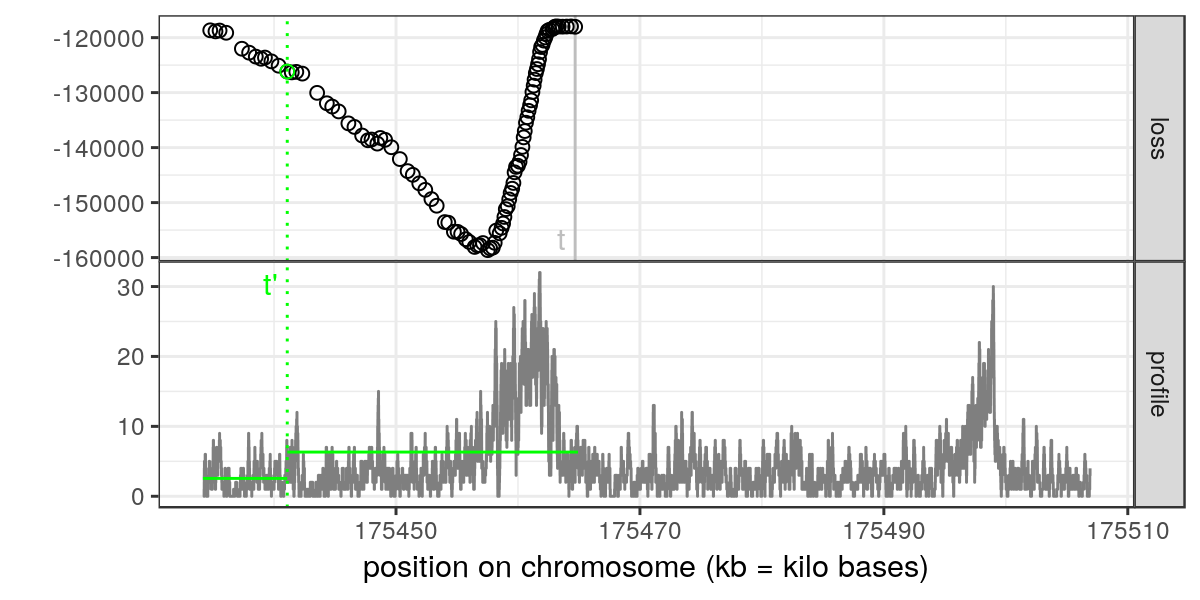
\includegraphics[width=\textwidth]{figure-dp-short-1.png}

$$
\mathcal L_{2, t} =
\min_{
  t' < t
}
\underbrace{
  \mathcal L_{1, t'}
}_{
  \text{optimal loss in 1 segment up to $t'$}
}
+
\underbrace{
  c_{(t', t]}
}_{
  \text{optimal loss of 2nd segment $(t', t]$}
}
$$

\end{frame}
 
\begin{frame}
\frametitle{Computation of optimal loss $\mathcal L_{s, t}$
  for $s=2$ segments up to data point $t < d$}
  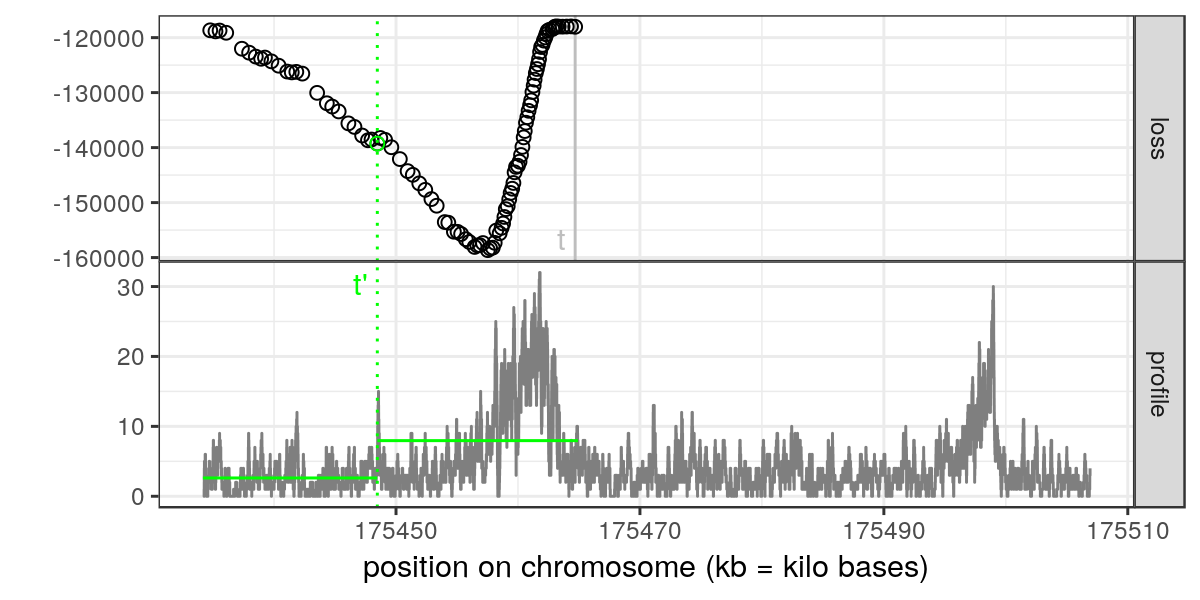
\includegraphics[width=\textwidth]{figure-dp-short-2.png}

$$
\mathcal L_{2, t} =
\min_{
  t' < t
}
\underbrace{
  \mathcal L_{1, t'}
}_{
  \text{optimal loss in 1 segment up to $t'$}
}
+
\underbrace{
  c_{(t', t]}
}_{
  \text{optimal loss of 2nd segment $(t', t]$}
}
$$

\end{frame}
 
\begin{frame}
\frametitle{Computation of optimal loss $\mathcal L_{s, t}$
  for $s=2$ segments up to data point $t < d$}
  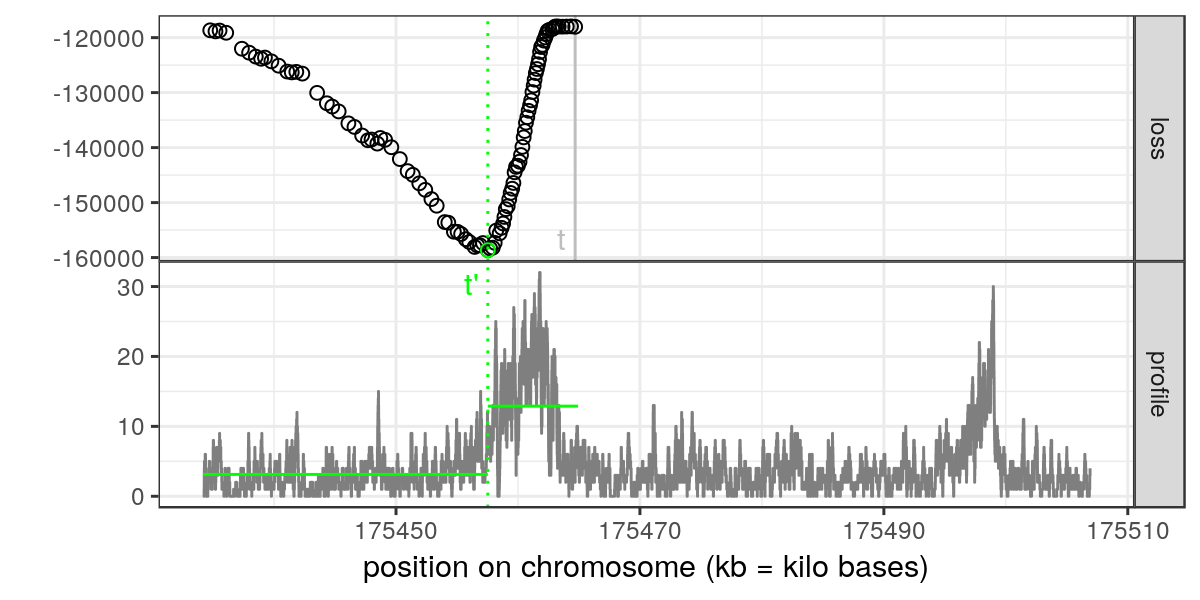
\includegraphics[width=\textwidth]{figure-dp-short-3.png}

$$
\mathcal L_{2, t} =
\min_{
  t' < t
}
\underbrace{
  \mathcal L_{1, t'}
}_{
  \text{optimal loss in 1 segment up to $t'$}
}
+
\underbrace{
  c_{(t', t]}
}_{
  \text{optimal loss of 2nd segment $(t', t]$}
}
$$

\end{frame}
 
\begin{frame}
\frametitle{Computation of optimal loss $\mathcal L_{s, t}$
  for $s=2$ segments up to data point $t < d$}
  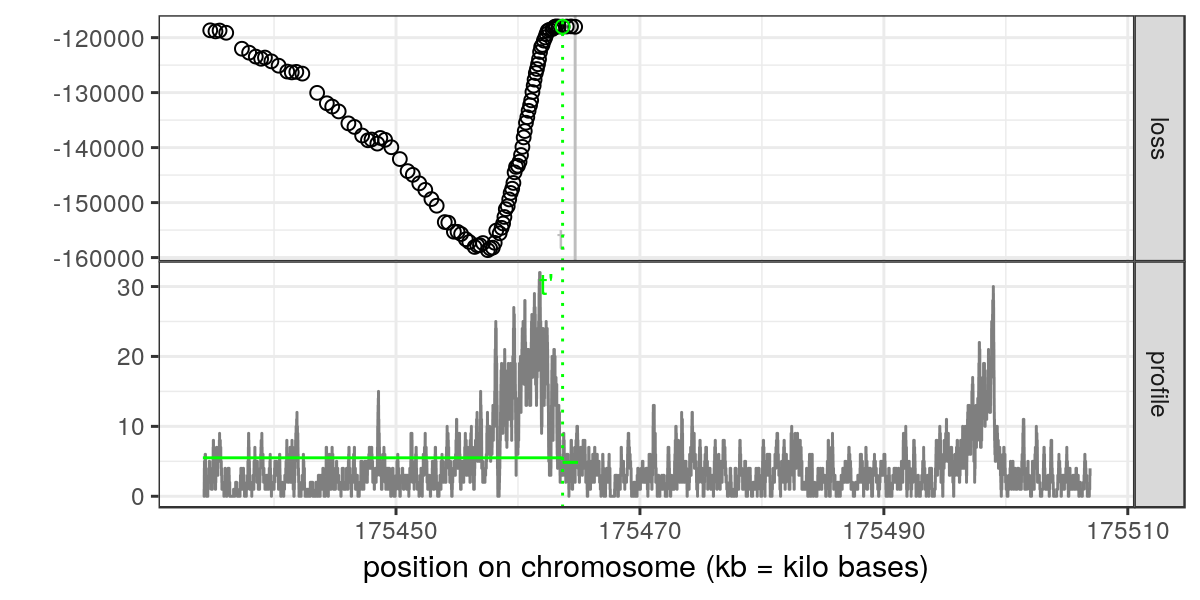
\includegraphics[width=\textwidth]{figure-dp-short-4.png}

$$
\mathcal L_{2, t} =
\min_{
  t' < t
}
\underbrace{
  \mathcal L_{1, t'}
}_{
  \text{optimal loss in 1 segment up to $t'$}
}
+
\underbrace{
  c_{(t', t]}
}_{
  \text{optimal loss of 2nd segment $(t', t]$}
}
$$

\end{frame}
